Over $1780$ random DAGs, $0.15$-strong faithfulness held in $56.2\%$;
Table~\ref{tab:main} and Table~\ref{tab:main-comparators} report the two
strata separately at $1000$ and $500$ instances, CERT-CD's own error types in
the first and the comparators' in the second, because a false edge or a wrong
arrow is not the same failure as a lost edge and the two are not a single
table's columns.

Where the premise holds, all four procedures behave. Where it fails---the
regime that breaks delete-on-non-rejection---SPRINT-CD loses a true edge in
$33.8\%$ of runs and PC in $48.2\%$ (Table~\ref{tab:main-comparators}), while
CERT-CD's adjacency certificates stay comfortably inside their
$\alpha_A = 0.05$ budget at $0.012$ ($[0.006, 0.026]$,
Table~\ref{tab:main}). Near-unfaithful instances cost the adjacency layer
power rather than validity: the affected pairs stay undecided instead of
being asserted wrongly. This is a within-stratum contrast for each method
against its own budget or its own failing behaviour, not a claim that
$0.012$ is smaller than $0.338$ in any sense that makes CERT-CD's adjacency
layer superior to SPRINT-CD's skeleton on a shared scale---the two numbers
answer different questions.

\paragraph{The orientation rate sits above budget on the failing stratum,
without our replication settling whether that is real.} The bolded entry in
Table~\ref{tab:main} is a wrong arrowhead in $29$ of $500$ runs, $0.058$ with
interval $[0.041, 0.082]$, against an orientation budget of $\alpha_D = 0.05$.
The interval contains the budget, and a one-sided binomial test against
$\alpha_D$ gives $p = 0.23$: at this replication count we cannot conclude
that the direction certificates fail to deliver the guarantee of
Theorem~\ref{thm:main} on this stratum. This number has a history worth
stating rather than hiding. A $20$-run check once reported $0/20$ here, and
we drew the wrong conclusion that the stratum was safe. A $250$-run check,
computed before we found and fixed the supremum-attainment defect
Remark~\ref{rem:supremum} describes, reported $20$ of $250$ with an interval
that excluded the budget, and an earlier version of this paper reported that
as a confirmed exceedance. The fix changes the fitting routine, not the
generating model or the stratification, and re-running the identical design
after the fix gives $16$ of $250$; the $500$-run design above, run
independently at higher replication, gives $29$ of $500$. Both post-fix point
estimates sit at or slightly above $0.05$; neither excludes it. We do not
know whether a small real exceedance survives on this stratum or whether two
point estimates landing on the high side is itself unremarkable at this
effect size---what the fix demonstrably removed was an artefact large enough
to look like proof of one.

The mechanism is the one Remark~\ref{rem:misspec} names, and it reaches the
direction certificate through the adjacency layer rather than independently of
it. The conditioning block $Z_{ij}$ is frozen to the pair's
\emph{already-certified} neighbours (Section~\ref{sec:freezing}). On a
near-unfaithful instance fewer neighbours have been certified by the time a
pair is opened, so $Z_{ij}$ more often omits a variable that is a parent of
$i$ or of $j$. The pair then has an uncontrolled common cause or an omitted
direct parent, the linear non-Gaussian model of
Section~\ref{sec:direction} is not the truth, and the domination step in the
proof of Proposition~\ref{prop:direction} has nothing to stand on.

We tested that explanation rather than asserting it. Over $250$ instances in
each stratum we recorded, for every certified arrowhead, whether the frozen
block $Z_{ij}$ contained every parent of $i$ and of $j$, and whether the
arrowhead was wrong. Table~\ref{tab:diag} reports the result. Note that these
are per-\emph{arrowhead} rates, whereas Table~\ref{tab:main} reports
per-\emph{run} rates.

\begin{table}[t]
\centering
\caption{Wrong-arrowhead rate by whether the frozen conditioning block
contained every parent of both endpoints, $250$ instances per stratum, Wilson
$95\%$ intervals. Rates are per certified arrowhead.}\label{tab:diag}
\footnotesize
\begin{tabular}{@{}llccc@{}}
\toprule
stratum & $Z_{ij}$ & arrowheads & wrong & rate \\
\midrule
premise holds & complete   & $486$ & $2$  & $0.004$ \tiny{[.001,.015]} \\
premise holds & incomplete & $224$ & $3$  & $0.013$ \tiny{[.005,.039]} \\
premise fails & complete   & $465$ & $3$  & $0.007$ \tiny{[.002,.019]} \\
premise fails & incomplete & $447$ & $22$ & $0.049$ \tiny{[.033,.073]} \\
\bottomrule
\end{tabular}
\end{table}

Both halves of the explanation hold. Incompleteness is more common where the
premise fails---$49.0\%$ of certified arrowheads against $31.5\%$ where it
holds (Fisher $p = 1.4\times10^{-12}$)---which is the certification-order
effect. And incompleteness is where the errors are: on the failing stratum the
wrong-arrowhead rate is $0.049$ with an incomplete block against $0.007$ with
a complete one, a factor of $7.6$ (Fisher $p = 5.5\times10^{-5}$), and $22$ of
the $25$ wrong arrowheads occur on pairs with an incomplete block. These are
per-arrowhead rates, not the quantity $\alpha_D$ bounds: $\alpha_D$ is a
whole-run, family-wise budget summed over all $d(d-1)$ direction nulls
(Section~\ref{sec:algo-desc}), so the two are not on a common scale and the
per-arrowhead rate being numerically smaller than $\alpha_D$ is not itself a
statement that any budget is respected. What the stratification does support
is the qualitative claim already made: the errors are not spread evenly but
concentrated on the incomplete-block cells, which is where
Theorem~\ref{thm:main}'s direction premise is violated.

\begin{figure}[t]
\centering
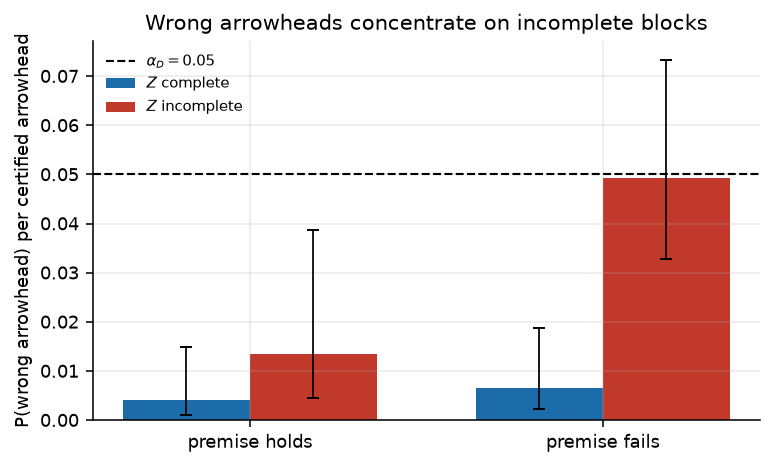
\includegraphics[width=0.72\textwidth]{figs/exp11_block_completeness.png}
\caption{Wrong-arrowhead rate by conditioning-block completeness, with Wilson
$95\%$ intervals. The dashed line marks $\alpha_D$'s numerical value for
scale only: $\alpha_D$ bounds the whole-run, family-wise probability of any
wrong arrowhead over all $d(d-1)$ direction nulls, not the per-arrowhead rate
plotted here, so a bar falling below the line is not a budget statement. The
exceedance in Table~\ref{tab:main} lives entirely in the incomplete-block bar
on the premise-failing stratum.}\label{fig:exp11}
\end{figure}

Figure~\ref{fig:exp11} plots the four cells at the same numerical scale as
$\alpha_D$, without claiming the two are the same quantity.

The exceedance in Table~\ref{tab:main} is therefore not a failure of
Proposition~\ref{prop:direction} or of its implementation. It is the
misspecification gap of Remark~\ref{rem:misspec} being opened by a specific,
identifiable mechanism, and it is reached through the algorithm's own
scheduling rather than through anything intrinsic to the direction null.


Two consequences should be stated plainly, and the first does not depend on
how the inconclusive test above eventually resolves. Theorem~\ref{thm:main}'s
direction clause is conditional on a premise---causal sufficiency for the pair
\emph{given the frozen block}---that the algorithm cannot verify and that is
correlated with faithfulness through the certification order. That is a
property of the proof, true whether or not this particular experiment's point
estimate turns out to sit significantly above $\alpha_D$. It is therefore not
the assumption-light guarantee the adjacency clause is, and the whole-graph
bound holds unconditionally only for adjacency, as Section~\ref{sec:intro}
now states.

Second, there is no cheap fix, and we record why rather than gesturing at one.
The obvious alternative---freezing $Z_{ij}$ to \emph{all} other variables
rather than to the certified neighbours, removing the dependence on
certification order---trades one failure for a worse one: with no
orientations available at freezing time, an all-variables block cannot
exclude a collider or a descendant of either endpoint, and conditioning on
either takes the pair outside \emph{both} branches of
Eqs.~\eqref{eq:fwd}--\eqref{eq:bwd}, so the certifying-null property fails
even when every true parent is present and the global model holds
everywhere. The certified-neighbour freeze used throughout this paper can
miss a true parent; the all-variables freeze can include a collider; neither
is a correct default, and we are not aware of a rule for $Z_{ij}$ that avoids
both failure modes with only the orientations available at the moment a pair
is certified. Closing this is, alongside the multiplicity gap of
Section~\ref{sec:multiplicity}, the open problem we consider most pressing.

Figure~\ref{fig:exp6} shows both panels: the validity comparison by stratum,
and what accumulates as $n$ grows.

\paragraph{What is certified.} On premise-satisfying instances at $n = 3000$,
$97\%$ of true edges are certified and $94\%$ are also oriented---so $97\%$ of
\emph{certified} edges carry a direction---against a Markov-equivalence-class
orientation ceiling of $28\%$, the fraction a CPDAG can orient at all on these
graphs. That gap is the practical content of the direction certificate: an
edge left undirected in the CPDAG is unorientable in principle by any
constraint-based method, and about $72\%$ of these edges are of that
kind.

The cost side of the same run is that $75\%$ of all pairs remain undecided at
$n = 3000$. Most of those pairs are genuinely non-adjacent---the graphs are
sparse---and CERT-CD is structurally unable to say so. A reader comparing
output sizes should keep this in view: PC returns a complete verdict on all
$10$ pairs, CERT-CD returns a verdict on about two or three.
